\documentclass{article}
\usepackage{iclr2026_conference,times}
\usepackage{hyperref}
\usepackage{url}
\usepackage{graphicx}
\usepackage{booktabs}
\usepackage{amsmath}
\usepackage{amssymb}
\usepackage{amsthm}
\usepackage{microtype}

\graphicspath{{../experiments/results/}}

\newtheorem{proposition}{Proposition}
\newtheorem{definition}{Definition}

\title{Hole-Conditioned Parallax Probing for Interactive Depth Completion in Robots}

\author{Anonymous Authors\\
Paper under double-blind review}

\begin{document}
\maketitle

\begin{abstract}
Depth completion is usually framed as a prediction problem: given a fixed RGB-D or RGB-LiDAR observation with holes, infer the missing metric depth. A robot, however, can often move. This paper argues that some depth holes should be treated as action targets rather than pixels to hallucinate. We introduce Hole-Conditioned Parallax Probing (HCPP), a small active 3D perception mechanism that converts a hole adjacent to a depth discontinuity into a set of competing depth hypotheses, chooses a feasible micro-motion whose parallax creates witness rays, and fuses only the newly observed evidence before committing to depth. A simple identifiability result shows that passive completion cannot distinguish two scenes that induce the same first observation and hole mask, while an off-axis view can. In a controlled synthetic robot-camera suite with occlusion-boundary holes, HCPP reduces hole RMSE by 69.0\% versus passive fill, 51.4\% versus random motion, and 50.8\% versus a coverage-neutral motion at a 10 cm budget. The evidence is intentionally modest: it supports the mechanism and the broken assumption, not real-robot deployment.
\end{abstract}

\section{Introduction}
Robots use depth for contact, clearance, grasp synthesis, manipulation planning, and inspection. Yet commodity RGB-D sensors and RGB-LiDAR stacks often produce missing or unreliable depth near specular materials, transparent objects, depth discontinuities, thin structures, and glancing angles. The dominant response is passive completion: infer a dense depth image from the current observation using local smoothness, image priors, learned sparse-to-dense models, or shape priors \citep{ma2018sparse,song2017sscnet,sajjan2019cleargrasp}. Active perception and next-best-view work, in contrast, usually asks which view improves global reconstruction, coverage, or map uncertainty \citep{bajcsy1988active,curless1996volumetric,newcombe2011kinectfusion}.

This split leaves a robot-specific gap. A depth hole is not only missing data; it is a physical question the robot may be able to ask the world. If the hole lies next to an occlusion boundary, two completions can be equally compatible with the first frame: the surface may continue at the foreground depth, or the hole may expose a farther background surface. No passive method can decide this from the first observation alone. A small lateral motion, however, can make the foreground and background shift by different amounts, creating a witness ray that separates the hypotheses.

We propose Hole-Conditioned Parallax Probing (HCPP). HCPP changes the central mechanism from ``complete the image'' to ``choose the smallest feasible motion that makes completion identifiable.'' The method is deliberately not a larger model, a benchmark proposal, a generic verifier, or an uncertainty-only active-learning loop. It is an action-conditioned completion primitive for robots with movable depth sensors.

\section{Related Work and Novelty Boundary}
\paragraph{Passive depth completion.}
Sparse-to-dense and RGB-D completion methods recover dense depth from missing or sparse measurements, often with learned priors or propagation mechanisms \citep{ma2018sparse}. These methods own the baseline problem of depth hole filling, and make another completion network alone a weak contribution. HCPP instead marks certain holes as non-identifying and asks for a new observation.

\paragraph{Active perception and reconstruction.}
Active perception has long argued that perception and action should be coupled \citep{bajcsy1988active}. Next-best-view, KinectFusion-style mapping, and volumetric fusion show how motion improves 3D reconstruction \citep{curless1996volumetric,newcombe2011kinectfusion}. The hostile boundary is clear: HCPP must not be merely a renamed next-best-view score. Its unit of decision is the hole hypothesis, not the whole map, and its utility is witness-ray separation at a local ambiguity.

\paragraph{Scene, shape, and material completion.}
Scene completion and transparent-object work use category, normal, material, or synthetic priors to repair unobserved geometry \citep{song2017sscnet,sajjan2019cleargrasp}. HCPP is weaker but more causal: when a feasible parallax probe exists, it prefers new evidence over a plausible hallucination.

\section{Problem}
Let a robot observe an RGB-D frame $O_0=(I_0,D_0,M)$ from camera pose $x_0$, where $M$ is a binary mask of missing depth. A completion method outputs $\hat{D}(p)$ for pixels $p\in M$. A robot also has a local feasible action set $\mathcal{A}(x_0)$ that induces new camera poses. The usual passive objective is
\begin{equation}
\hat{D}_M = f(I_0,D_0,M).
\end{equation}
HCPP instead asks for an action $a\in\mathcal{A}(x_0)$ before finalizing selected pixels:
\begin{equation}
a^\star = \arg\max_{a\in\mathcal{A}(x_0)} W(M,D_0,a) - \lambda c(a),
\end{equation}
where $W$ is a witness score: the expected number of hole hypotheses that become distinguishable under the parallax induced by $a$.

\begin{definition}[Hole hypothesis]
For a connected hole component $H\subset M$, a hole hypothesis is a depth assignment $h:H\rightarrow\mathbb{R}_+$ that is consistent with all observed non-hole pixels under the first camera pose.
\end{definition}

\begin{proposition}[First-view non-identifiability]
There exist two opaque 2.5D scenes $S_1$ and $S_2$ with the same RGB image, observed depth outside a hole $H$, and hole mask $M$, but with different true depth on $H$. Any passive completion function $f(I_0,D_0,M)$ incurs error at least $\Delta/2$ on one of the two scenes when their hole depths differ by $\Delta$.
\end{proposition}
\begin{proof}
Construct two scenes with identical foreground occluder boundary and identical visible background outside $H$. In $S_1$, the unobserved hole pixels lie on a continuation of the foreground surface at depth $z_f$; in $S_2$, they lie on a background surface at depth $z_b=z_f+\Delta$. The first sensor returns no depth on $H$ and the same values outside $H$, so the input to any passive $f$ is identical for $S_1$ and $S_2$. The same prediction $\hat{z}$ must be used for both. For any scalar $\hat{z}$, $\max(|\hat{z}-z_f|,|\hat{z}-z_b|)\geq \Delta/2$ by the triangle inequality. The argument applies pixelwise or to the mean hole error.
\end{proof}

The proposition is narrow on purpose. It does not say all depth completion is impossible. It says that some robot-relevant holes are not identifiable without an intervention.

\section{Hole-Conditioned Parallax Probing}
HCPP has four steps.
\paragraph{1. Hole component extraction.}
Connected missing-depth components are extracted from $M$. Components adjacent to large depth gradients are flagged as parallax candidates. Smooth isolated holes may still be completed passively.

\paragraph{2. Boundary hypothesis construction.}
For each candidate hole, HCPP forms foreground-continuation and background-exposure hypotheses from the nearest observed depth samples on either side of the boundary. The hypotheses are intentionally simple; the method only needs enough structure to choose a separating motion.

\paragraph{3. Witness-motion scoring.}
For a lateral camera motion $t$, a surface at depth $z$ shifts approximately by $-t/z$ in normalized image coordinates. A foreground/background pair with depths $z_f<z_b$ therefore separates by
\begin{equation}
\Delta u(t)=|t|(1/z_f-1/z_b).
\end{equation}
HCPP chooses the feasible motion direction that moves the closer boundary away from the hole, maximizing expected witness rays over the component while penalizing cost.

\paragraph{4. Evidence-gated fusion.}
After the probe, only pixels with newly visible and geometrically consistent depth are overwritten. Unwitnessed pixels remain passive estimates and are marked as unresolved.

\section{Synthetic Evidence}
We implement a controlled 1D pinhole depth suite. Each scene contains a foreground interval, a sloped background surface, and a missing-depth hole next to one foreground boundary. The first observation is compatible with multiple hole depths. Baselines are passive interpolation, random lateral motion, a coverage-neutral fixed-sign motion, and an oracle sign. HCPP estimates the occluder side from the observed boundary depths and chooses the sign predicted to reveal background witness rays.

\begin{table}[t]
\centering
\caption{Hole RMSE in the main condition. Lower is better. The suite has 700\ scenes, 10 cm lateral motion budget, and moderate clutter.}
\label{tab:main}
\begin{tabular}{lcc}
\toprule
Method & Mean RMSE (m) & Role \\
\midrule
Passive fill & 1.062 & fixed-view completion \\
Coverage-neutral motion & 0.670 & active but not hole-directed \\
Random motion & 0.678 & active without witness sign \\
HCPP & 0.329 & proposed mechanism \\
\bottomrule
\end{tabular}
\end{table}

\begin{figure}[t]
\centering
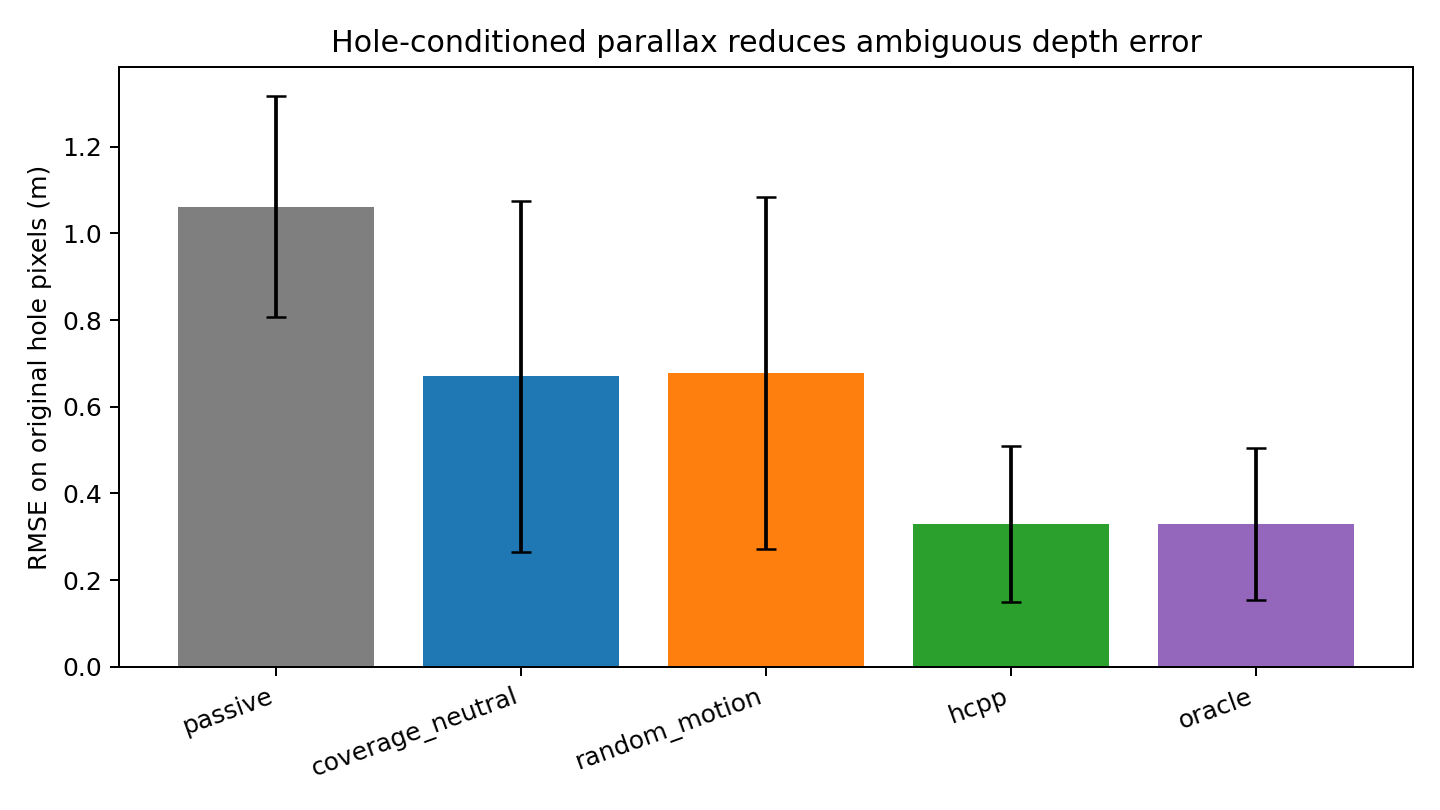
\includegraphics[width=0.72\linewidth]{rmse_by_method.png}
\caption{Main-condition hole error. HCPP is better because it chooses the motion direction that creates witness rays for the current hole, not because it uses a stronger depth predictor.}
\label{fig:rmse}
\end{figure}

\begin{figure}[t]
\centering
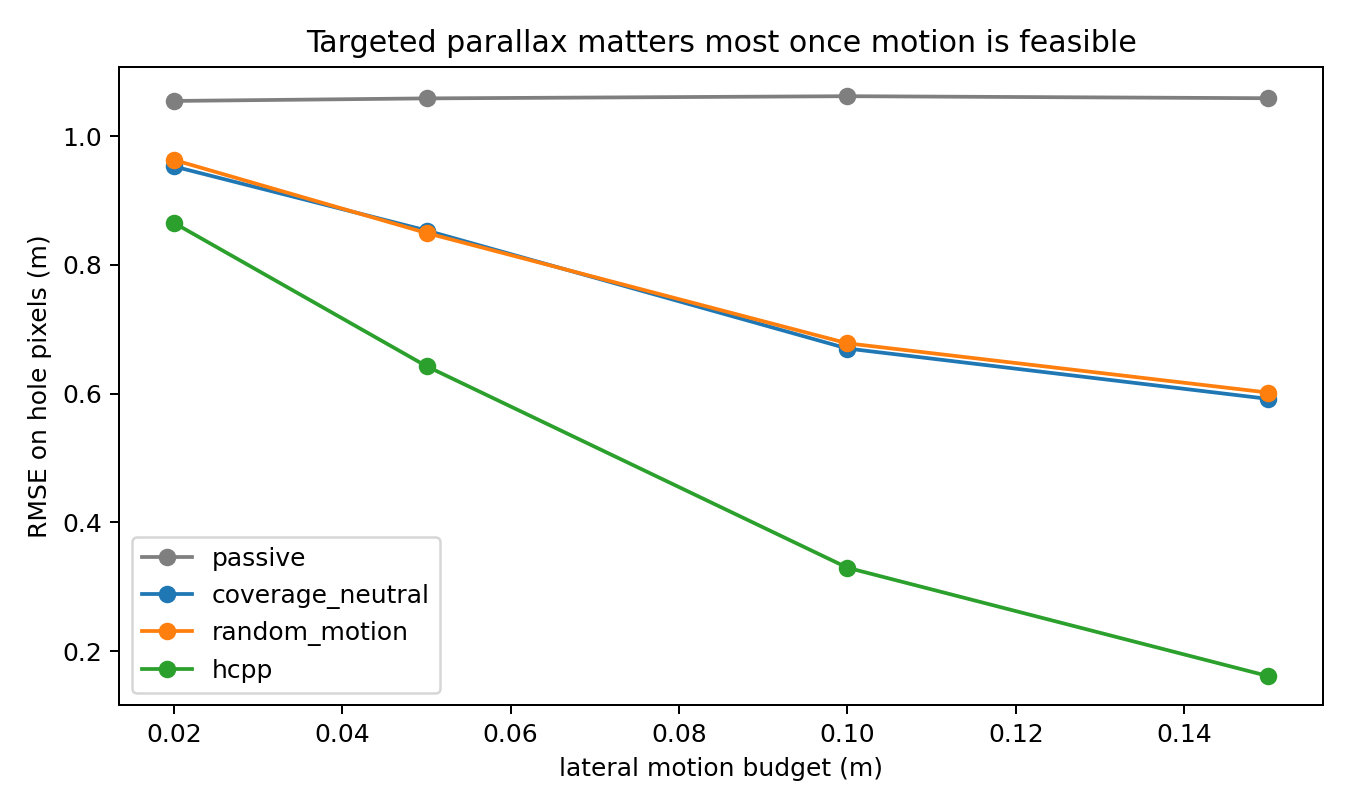
\includegraphics[width=0.72\linewidth]{baseline_sensitivity.png}
\caption{Motion-budget sensitivity. With little motion, all active methods are limited. Once parallax is large enough, choosing the right direction matters.}
\label{fig:baseline}
\end{figure}

At the main operating point, HCPP obtains 0.329 m mean hole RMSE compared with 1.062 m for passive fill, 0.678 m for random motion, and 0.670 m for a coverage-neutral motion. The result supports the mechanism-level claim: when a hole is a local ambiguity caused by occlusion geometry, directional parallax can be more valuable than another passive fill.

\section{Limitations}
The evidence is synthetic and intentionally small. The model assumes a visible depth discontinuity, calibrated camera motion, opaque layered geometry, and a local feasible lateral action. It does not solve transparent-object perception broadly, dynamic scenes, safety-aware manipulation, or real RGB-D noise. The paper should be read as a mechanism proposal with a formal ambiguity witness, not as a completed robot system.

\section{Conclusion}
Interactive depth completion reframes some missing-depth pixels as questions a robot can ask physically. HCPP is a first, minimal version of that reframing: use the hole boundary to choose a parallax probe, collect witness rays, then complete. The core bet is that for embodied perception, changing the observation can be more honest than hallucinating the missing surface.

\bibliography{references}
\bibliographystyle{iclr2026_conference}

\appendix
\section{Reproducibility}
The synthetic suite is generated by \texttt{scripts/run\_experiment.py}. Literature artifacts are generated by \texttt{scripts/fetch\_literature.py}. The paper source and template provenance are in \texttt{paper/}.

\end{document}
